\chapter{Stworzony system weryfikacji mówcy}\label{chap:badania}

\section{Przetworzenie danych}
\label{sec:data_wrangling}

Nagrania \techname{RedDots} zostały przetworzone w~ten sposób:

\begin{itemize}
    \item Przeprowadzana jest procedura \shortcut{VAD} (\foreign{voice activity detection}), czyli wyodrębnianie
        fragmentów nagrania zawierających sygnał mowy, za pomocą pakietu \techname{webrtcvad}. Użyty parametr
        agresji $2$. Z~każdego nagrania zostały usunięte ramki bezpośrednio z~początku i~z końca, które zostały
        uznane za ciche.
    \item Dla każdego obciętego nagrania obliczone zostały \shortcut{MFCC} korzystając z~metody z
        pakietu \techname{python-speech-features}. Analizę przeprowadzono w~oknach $25$ms z~$10$ms skokiem.
        Użyto okna Hamminga. Utworzono $26$ filtrów pokrywających częstotliwości nagrania i~zachowano z~nich
        $13$. Użyto filtru \foreign{preemphasis} z~parametrem $0.97$. Wynikiem jest $13$ współczynników.
    \item Dla każdej ramki obliczono cechy delta i~delta-delta z~użyciem pakietu \techname{python-speech-features}.
        Cechy te obliczono biorąc pod uwagę sąsiedztwo $4$ ramek przed i~$4$ ramek po danej ramce.
    \item Bardzo krótkie nagrania, składające się z~mniej niż $85$ ramek, zostały odrzucone. Kilka nagrań miało
        nawet długość $1$ ramki. Próg został wyznaczony przez zbadanie jakiej długości są nagrania. Między $85$
        i~krótszymi jest skok, więc uznano je za anomalie.
\end{itemize}

Wykorzystano słownik \techname{CMUDict} do zamiany wszystkich transkrypcji z~\techname{RedDots} na listy 39 fonemów
używanych w~języku angielskim. Zignorowano przy tym akcenty. Części nagrań nie udało się zamienić, gdyż
zawierały treść w~innym języku, i~one nie będą używane w~modelach wykorzystujących fonemy.

\section{Wykorzystane modele}
\label{sec:data_models}

W ramach pracy utworzone zostały trzy modele do weryfikacji mówcy. Zostały one tutaj opisane.

\subsectionex{Model GMM-UBM}{Mikstury gaussowskie z~uniwersalnym modelem tła}
\label{sec:gmm_ubm}

System \shortcut{GMM-UBM} jest wzorowany na tym opisanym w~pracy \cite{utteranceVerificationFor}. Posłużono
się również parametrami z~tej pracy.

Wpierw zebrano wszystkie dane ze zbioru \techname{RedDots}, które nie są użyte w~żadnym teście. Dopasowano
do nich model tła, który jest miksturą 512 dystrybucji normalnych. Założono, że cechy są nieskorelowane
i macierz kowariancji w~miksturach jest diagonalna.

W ramach zapisów model tła jest kopiowany i~\shortcut{MAP}-adaptowany z~\foreign{relevance factor} równym $3.0$
dla nagrań rejestracyjnych danego mówcy. Dodatkowo dla każdej grupy nagrań o~tej samej treści również tworzona
jest kopia modelu tła i~\shortcut{MAP} adaptowana w~ten sam sposób do nagrań z~tej grupy.

W czasie testów dla każdego nagrania liczone jest prawdopodobieństwo, że nagranie pochodzi z~modelu tła,
z \shortcut{GMM} mówcy, który jest oczekiwany w~weryfikacji i~z \shortcut{GMM} zdania, które jest oczekiwane.
Na podstawie tych wartości liczone są prawdopodobieństwa, że mówca i~treść są poprawne jako stosunek prawdopodobieństw.

$$S_{sp}(x) = \frac{P(\theta_{sp} | x)}{max(P(\theta_{sp} | x), P(\theta_{UBM} | x))}$$
$$S_{st}(x) = \frac{P(\theta_{st} | x)}{max(P(\theta_{st} | x), P(\theta_{UBM} | x))}$$
$$S_{both}(x) = S_{sp}(x) S_{st}(x)$$

\subsectionex{Model HMM-GMM}{Ukryty model Markowa z~emisjami w~postaci mikstur gaussowskich}
\label{sec:hmm_gmm}

Ten model jest wzorowany na modelu opisanym w~pracy \cite{comparisonOfMultiple}. Wykorzystuje
system rozpoznawania mowy do określenia, które ramki zawierają które fonemy. System ten
to ukryty łańcuch Markowa, w~który każdy fonem jest reprezentowany przez trzy stany. Został
użyty model monofonemowy. Dla wypowiedzi w~zbiorze znany jest ciąg fonemów, gdyż
\techname{RedDots} zawiera transkrypcje, które następnie zostały zamienione na fonemy
przez odszukanie odpowiednich słów w~słowniku \techname{CMUDict}. Dla każdej wypowiedzi
budowany jest \shortcut{HMM} przez złączenie odpowiednich trójek stanów zgodnie z~kolejnością
fonemów w~wypowiedzi. Tworzony jest łańcuch z~przejściami typu \foreign{beads-on-string}.

Dla każdego mówcy i~tła budowany jest zestaw mieszanin \shortcut{GMM}, po jednej na stan \shortcut{HMM},
a zatem po trzy na fonem. Każda mikstura składa się z~$8$ dystrybucji z~diagonalną macierzą kowariancji.

Parametry podsystemu rozpoznawania mowy są wyznaczane tak, że najpierw do wszystkich danych
dopasowywana jest mała 8 składnikowa mikstura tła. Następnie budowane są wszystkie trójki \shortcut{GMM}
odpowiadające fonemom. Potem dla każdej wypowiedzi budowany jest model Markowa przez połączenie odpowiednich
trójek zgodnie ze znanym ciągiem fonemów danej wypowiedzi. Korzystając z~\shortcut{HMM} i~algorytmu Viterbiego
ramki nagrania są przyporządkowywane do części fonemów. Algorytm jest zmodyfikowany, by dawał wyższe prawdopodobieństwo
podziałowi, w~którym każdemu ukrytemu stanowi odpowiada ta sama liczba ramek. To samo jest robione dla innych nagrań.
Następnie parametry trójek \shortcut{GMM} są dopasowywane przez \shortcut{EM} do ramek, które zostały im przypisane.
Po ustaleniu parametrów mikstur, ramki są przypisywane ponownie z~użyciem algorytmu Viterbiego i~proces jest ponawiany.

Rejestracje wyglądają tak, że dla każdego mówcy jest budowany jego zestaw trójek \shortcut{GMM}.
Wypowiedzi rejestracyjne danego mówcy są przyporządkowywane
częściom fonemów z~użyciem algorytmu Viterbiego przez opisane \shortcut{HMM}.
Używając tego przyporządkowania mikstury tła są \shortcut{MAP} adaptowane do nagrań danego mówcy.

Testy wyglądają podobnie. Najpierw z~użyciem systemu rozpoznawania mowy i~algorytmu Viterbiego znajdowane
jest, które ramki zawierają które części fonemów. Następnie dla każdej ramki obliczany jest logarytm prawdopodobieństwa,
iż pochodzi ona z~odpowiedniej mikstury mówcy i~odpowiedniej mikstury tła. Sumując je uzyskiwany jest wynik dla mikstur
mówcy i~mikstur tła. Wynik weryfikacji mówcy obliczany jest jako stosunek tych prawdopodobieństw. Treść
nagrania nie jest osobno sprawdzana.

$$S_{sp}(x) = exp(\sum_{x_i \in x} (log P(\theta_{sp} | x_i) - max(log P(\theta_{sp} | x_i), log P(\theta_{UBM} | x_i))))$$

\subsectionex{Model DNN-GMM}{Głęboka sieć neuronowa do dopasowania ramek, ocena miksturami gaussowskimi}
\label{sec:dnn_gmm}

W tym modelu wykorzystano głęboką sieć neuronową do rozpoznawania tekstu taką jak opisano w~pracy \cite{endToEnd}.
Sieć składa się z~pięciu warstw, w~tym jednej rekurencyjnej warstwy \shortcut{LSTM}.
Wytrenowanie tej sieci wymaga niestety ogromnej ilości danych i~czasu. Z~raportów innych osób wynikało, że na
zwykłym komputerze pojedyncza epoka nauki może zająć nawet dwa tygodnie. Z~tego powodu wykorzystany został
gotowy model stworzony przez organizację \techname{Mozilla}.

Model ten został wytrenowany na ok. 2500 godzinach nagrań ze zbiorów \techname{WSJ}, \techname{Switchboard}
i \techname{Fisher}. Warto zauważyć, że autorzy cytowanej pracy z~\techname{Baidu} poza tymi zbiorami użyli
dodatkowo własnego, zamkniętego zbioru 5000 godzin nagrań. Sieć ta przyjmuje kolejne ramki, przy czym muszą
one być wstępnie przetworzone do współczynników \shortcut{MFCC}. Dla każdej chwili zwracany jest wektor 28 liczb,
które odpowiadają 25 literom alfabetu, przerwie, apostrofowi i~szumowi.

Podobnie jak w~\shortcut{HMM-GMM} dla każdego nagrania znamy treść i~z wykorzystaniem systemu rozpoznawania
mowy przyporządkowujemy ramki literom. Istotna różnica jest taka, że tutaj system rozpoznawania mowy zwraca
tekst, nie sekwencje fonemów, co dla naszych potrzeb jest niepożądane. Gdyby trenować model od podstaw na
potrzeby rozpoznawania mówcy warto byłoby zmienić ten aspekt. Do przypisania ramek wykorzystano odpowiednio
dostosowany algorytm Viterbiego. Wyjścia sieci są w~nim znormalizowane do przedziału $[0.0, 1.0]$ i~traktowane
jako prawdopodobieństwa emisji danej ramki w~kolejnych stanach ukrytych. Stany ukryte są tożsame z~literami
i algorytm wymusza, by zmieniały się zgodnie ze znaną treścią oraz by wszystkie litery się pojawiły.
W przypadku, gdy największe prawdopodobieństwo przypada na szum algorytm pomija ramkę. Wynikiem
jest przypisanie do niektórych ramek liter oraz zwrócenie prawdopodobieństwa danej sekwencji - jak jest
bardzo małe to prawdopodobnie spodziewana treść i~treść na nagraniu się różnią.

Trening wygląda analogicznie jak opisano w~\shortcut{HMM-GMM}. To znaczy korzystając z~przypisania ramek
zwróconego przez \shortcut{DNN}, tworzy się szereg \shortcut{GMM} z~$8$ składnikami mikstury
i macierzami diagonalnymi, po jednym na literę. Następnie wyznaczane są ich parametry, by
maksymalizowały prawdopodobieństwo wystąpienia
ramek z~ich klasy. Rejestracja wygląda tak samo, tylko \shortcut{MAP} adaptuje modele tła do
mniejszej liczby nagrań rejestracyjnych mówcy.

Metoda testowania ponownie polega na policzeniu stosunku prawdopodobieństw między \shortcut{GMM} mówcy, a~tła.
Wynik jest sumowany dla wszystkich ramek, które mają przypisane litery. Weryfikacja treści nagrania
bazuje na prawdopodobieństwie zwróconym przez algorytm Viterbiego, czyli prawdopodobieństwie najbardziej
prawdopodobnej sekwencji przyporządkowań liter do ramek, w~której litery zgadzają się z~transkrypcją.

\section{Wyniki testów}
\label{sec:test_results}

W celu oceny systemów wykonano pierwsze zadanie zdefiniowane w~zbiorze \techname{RedDots}. Każdy z~modeli został
wykorzystany do zapisów mówców, a~następnie do testów. Algorytm wykorzystania modeli wraz ze wszystkimi parametrami
zapisany jest w~plikach \techname{Jupyter}, co powinno uczynić wyniki łatwymi do odtworzenia,
choć powtórzenie obliczeń może zająć dużo czasu.
Wyniki w~postaci krzywej \shortcut{ROC}, \shortcut{EER} i~\shortcut{AUC} zapisano w~poniższej tabeli
i zwizualizowano pod tabelą.

\begin{table}[H]
    \centering
    \caption{Wyniki \shortcut{EER} i~\shortcut{AUC} uzyskane przez modele \shortcut{GMM-UBM}, \shortcut{HMM-GMM}, \shortcut{DNN-GMM} na pierwszym zadaniu zdefiniowanym w~zbiorze \techname{RedDots}}
    \label{tab:all_results}
    \small
    \tabulinesep =_3pt^3pt
    \begin{tabu}{l*{6}{r}}
        \multirow{2}{*}{Model} & \multicolumn{2}{c}{Tylko mówca} & \multicolumn{2}{c}{Tylko treść} & \multicolumn{2}{c}{Mówca i~treść}
        \\
        & \shortcut{EER} & \shortcut{AUC} & \shortcut{EER} & \shortcut{AUC} & \shortcut{EER} & \shortcut{AUC}
        \\ \midrule
        \shortcut{GMM-UBM} & 4.69\% & 97.56\% & 6.04\% & 97.82\% & 3.20\% & 99.04\%
        \\
        \shortcut{HMM-GMM} & 15.86\% & 92.73\% & - & - & 5.16\% & 98.32\%
        \\
        \shortcut{DNN-GMM} & 39.51\% & 65.12\% & 17.65\% & 86.73\% & 24.24\% & 84.38\%
        \\
    \end{tabu}
\end{table}

\begin{figure}[H]
    \centering
    \begin{minipage}{.5\textwidth}
        \centering
        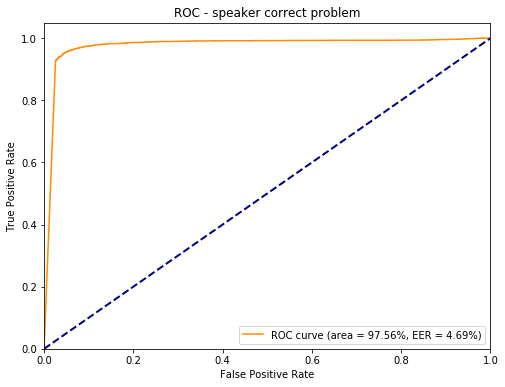
\includegraphics[width=0.8\textwidth]{images/4_3_gmm_roc_speaker}
        \label{fig:4_3_gmm_roc_speaker}
    \end{minipage}%
    \begin{minipage}{.5\textwidth}
        \centering
        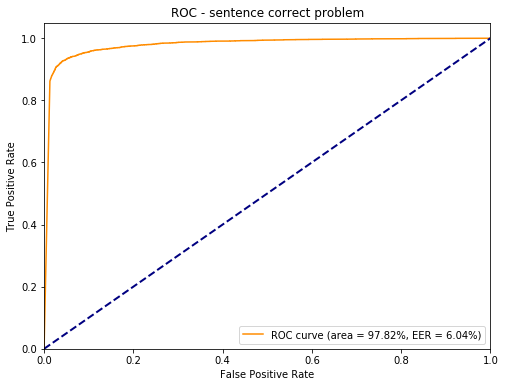
\includegraphics[width=0.8\textwidth]{images/4_3_gmm_roc_sentence}
        \label{fig:4_3_gmm_roc_sentence}
    \end{minipage}
    \caption{Wykresy krzywej \shortcut{ROC} dla \shortcut{GMM-UBM}, pierwszego zadania \techname{RedDots} i~przypadków weryfikacji mówcy oraz weryfikacji treści}
\end{figure}

\begin{figure}[H]
    \centering
    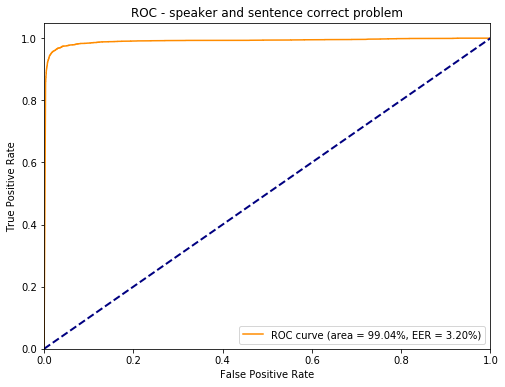
\includegraphics[width=0.6\textwidth]{images/4_3_gmm_roc_both}
    \caption{Wykres krzywej \shortcut{ROC} dla \shortcut{GMM-UBM}, pierwszego zadania \techname{RedDots} i~jednoczesnej weryfikacji mówcy i~treści}
    \label{fig:4_3_gmm_roc_both}
\end{figure}

\begin{figure}[H]
    \centering
    \begin{minipage}{.5\textwidth}
        \centering
        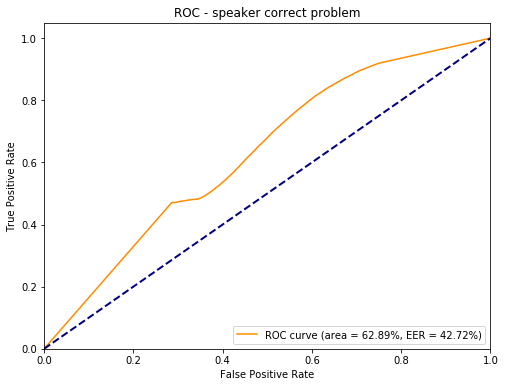
\includegraphics[width=0.9\textwidth]{images/4_3_dnn_roc_speaker}
        \label{fig:4_3_dnn_roc_speaker}
    \end{minipage}%
    \begin{minipage}{.5\textwidth}
        \centering
        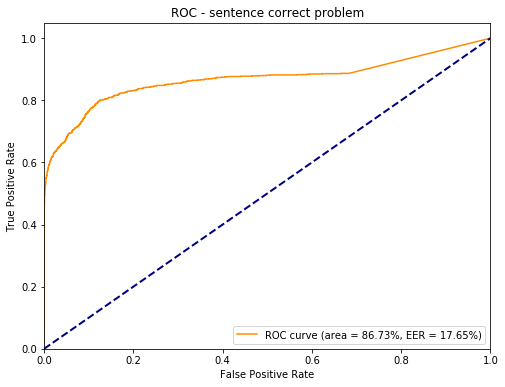
\includegraphics[width=0.9\textwidth]{images/4_3_dnn_roc_sentence}
        \label{fig:4_3_dnn_roc_sentence}
    \end{minipage}%
    \caption{Wykresy krzywej \shortcut{ROC} dla \shortcut{DNN-GMM}, pierwszego zadania \techname{RedDots} i~przypadków weryfikacji mówcy oraz weryfikacji treści}
\end{figure}

\begin{figure}[H]
    \centering
    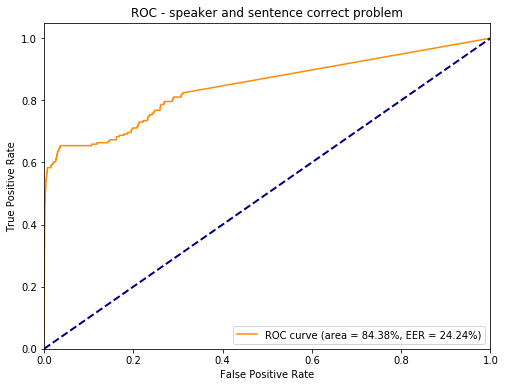
\includegraphics[width=0.6\textwidth]{images/4_3_dnn_roc_both}
    \caption{Wykres krzywej \shortcut{ROC} dla \shortcut{DNN-GMM}, pierwszego zadania \techname{RedDots} i~jednoczesnej weryfikacji mówcy i~treści}
    \label{fig:4_3_dnn_roc_both}
\end{figure}

\begin{figure}[H]
    \centering
    \begin{minipage}{.5\textwidth}
        \centering
        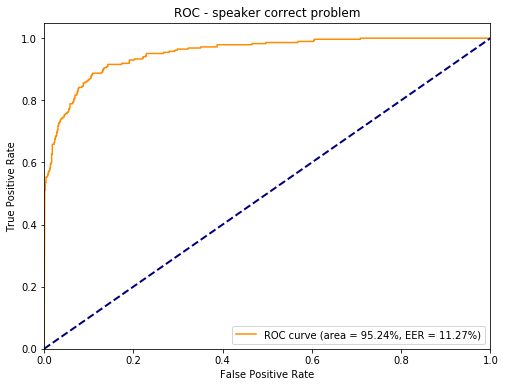
\includegraphics[width=0.9\textwidth]{images/4_3_hmm_roc_speaker}
        \label{fig:4_3_hmm_roc_speaker}
    \end{minipage}%
    \begin{minipage}{.5\textwidth}
        \centering
        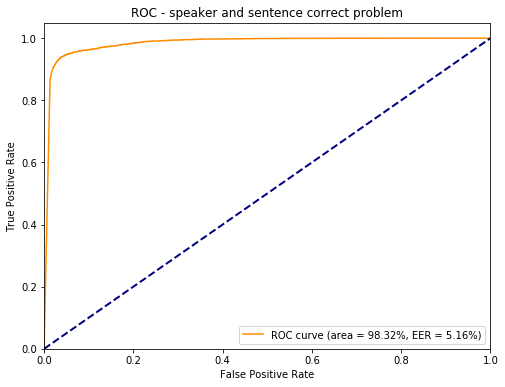
\includegraphics[width=0.9\textwidth]{images/4_3_hmm_roc_both}
        \label{fig:4_3_hmm_roc_both}
    \end{minipage}
    \caption{Wykresy krzywej \shortcut{ROC} dla \shortcut{HMM-GMM}, pierwszego zadania \techname{RedDots} i~przypadków weryfikacji mówcy oraz jednoczesnej weryfikacji mówcy i~treści}
\end{figure}

